\section{Design the control circuit using three variables: PWM, Direction, Brake as inputs}
    \begin{figure}[H]
        \centering
        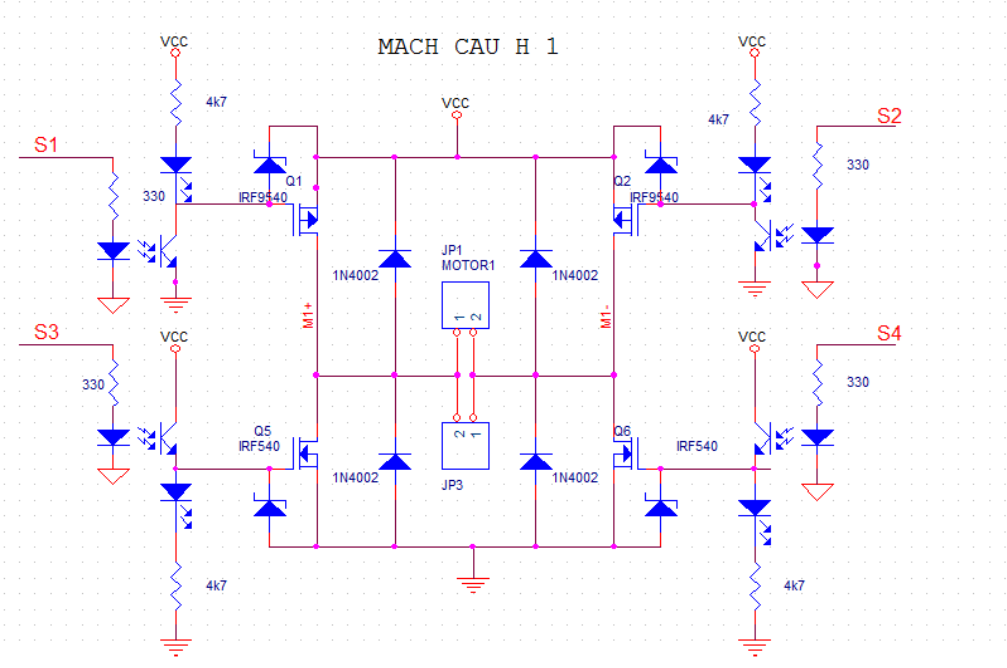
\includegraphics[width=0.9\textwidth]{pictures/3_diagram.png}
        \caption{Sơ đồ mạch cầu H}
        \label{fig:3_diagram}
    \end{figure}
    \begin{table}[H]
        \centering
        \begin{tabular}{|c|c|c|c|c|c|c|c|}
            \hline
            PWM1 & PWM2 & BRAKE & S1 & S2 & S3 & S4 & TRANG THAI MOTOR \\
            \hline
            0 & 1 & 1 & 1 & 0 & 0 & 1 & QUAY CHIEU THUAN \\
            \hline
            0 & 0 & 1 & 0 & 1 & 1 & 0 & QUAY CHIEU NGHICH \\
            \hline
            X & X & 0 & 1 & 1 & 0 & 0 & THANG \\
            \hline
            1 & X & 1 & 0 & 0 & 0 & 0 & DUNG QUAY \\
            \hline
        \end{tabular}\\
        \caption{Bảng trạng thái tín hiệu các biến}
        \label{tab:motor_states}
    \end{table}
    \subsection{Tìm mối quan hệ giữa 3 biến đầu vào với S1, S2, S3 và S4}
        \subsubsection{Áp dụng bìa Karnaugh để tìm S1}
            \begin{centering}
                \begin{tabular}{|c|c|c|c|c|}
                    \hline
                    \diagbox{Z}{XY} & 00 & 01 & 11 & 10 \\
                    \hline
                    0 & 1 & 1 & 1 & 1 \\
                    \hline
                    1 &  & 1 &  &  \\
                    \hline
                \end{tabular} \\
            \end{centering}
            $\Rightarrow S1 = \overline{Z} + \overline{X}.Y$ 
        \subsubsection{Áp dụng bìa Karnaugh để tìm S2}
            \begin{centering}
                \begin{tabular}{|c|c|c|c|c|}
                    \hline
                    \diagbox{Z}{X} & 00 & 01 & 11 & 10 \\
                    \hline
                    0 & 1 & 1 & 1 & 1 \\
                    \hline
                    1 & 1 &  &  &  \\
                    \hline
                \end{tabular}\\
            \end{centering}
            $\Rightarrow S2 = \overline{Z} + \overline{X}.\overline{Y}$ 
        \subsubsection{Áp dụng bìa Karnaugh để tìm S3}
            \begin{centering}
                \begin{tabular}{|c|c|c|c|c|}
                    \hline
                    \diagbox{Z}{XY} & 00 & 01 & 11 & 10 \\
                    \hline
                    0 &  &  &  &  \\
                    \hline
                    1 & 1 &  &  &  \\
                    \hline
                \end{tabular}\\
            \end{centering}
            $\Rightarrow S3 = \overline{X}.\overline{Y}.Z$ \\
        \subsubsection{Áp dụng bìa Karnaugh để tìm S4}
            \begin{centering}
                \begin{tabular}{|c|c|c|c|c|}
                    \hline
                    \diagbox{Z}{XY} & 00 & 01 & 11 & 10 \\
                    \hline
                    0 &  &  &  &  \\
                    \hline
                    1 &  & 1 &  &  \\
                    \hline
                \end{tabular}\\
            \end{centering}
            $\Rightarrow S4 = \overline{X}.Y.Z$ \\
    \subsection{Vẽ mạch bằng phần mềm Proteus.}
        \begin{itemize}
            \item Mạch được mô phỏng trên phần mềm Proteus.
            \item Các linh kiện được sử dụng: AND, NOT, OR, LOGICPROBE, LOGICSTATE. 
            \item Kết quả mô phỏng theo hàng thứ nhất của bảng \ref{tab:motor_states}:
                \begin{figure}[H]
                    \centering
                    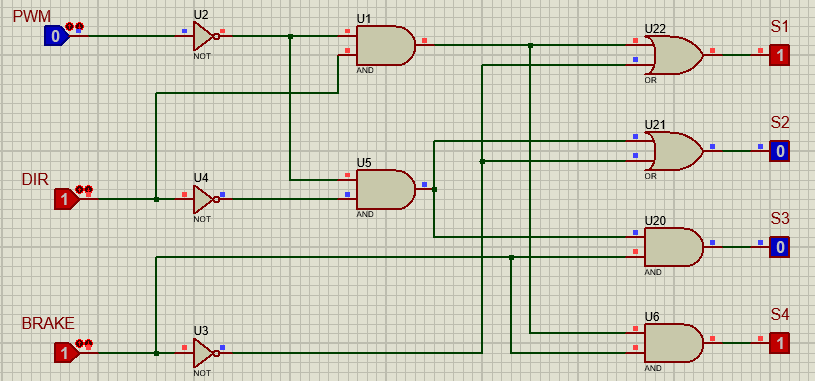
\includegraphics[width=0.6\textwidth]{pictures/3_result1.png}
                    \caption{Trường hợp 1: PWM1 = 0, PWM2 = 1, BRAKE = 1}
                \end{figure} 
            \item Kết quả mô phỏng theo hàng thứ hai của bảng \ref{tab:motor_states}:
                 \begin{figure}[H]
                    \centering
                    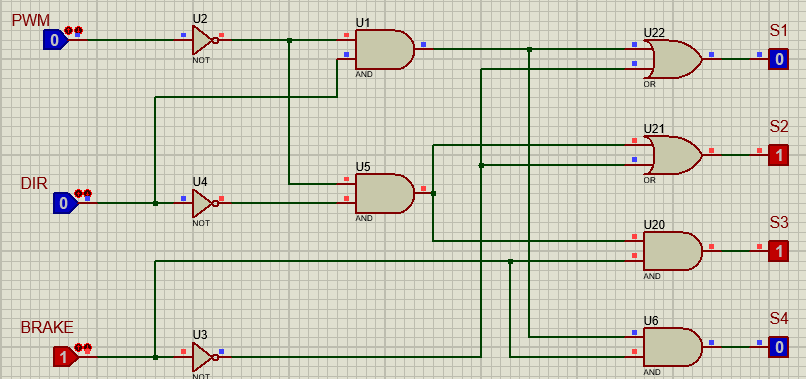
\includegraphics[width=0.6\textwidth]{pictures/3_result2.png}
                    \caption{Trường hợp 2: PWM1 = 0, PWM2 = 0, BRAKE = 1}
                \end{figure}
            \item Kết quả mô phỏng theo 1 trong các trường hợp của hàng thứ ba của bảng \ref{tab:motor_states}:
                \begin{figure}[H]
                    \centering
                    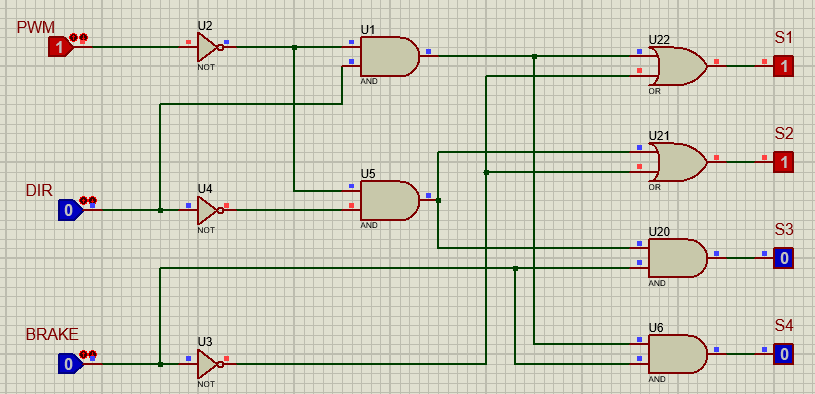
\includegraphics[width=0.6\textwidth]{pictures/3_result3.png}
                    \caption{Trường hợp 3: PWM1 = 1, PWM2 = 0, BRAKE = 0}
                \end{figure}
            \item Kết quả mô phỏng theo 1 trong các trường hợp của hàng thứ tư của bảng \ref{tab:motor_states}:
                \begin{figure}[H]
                    \centering
                    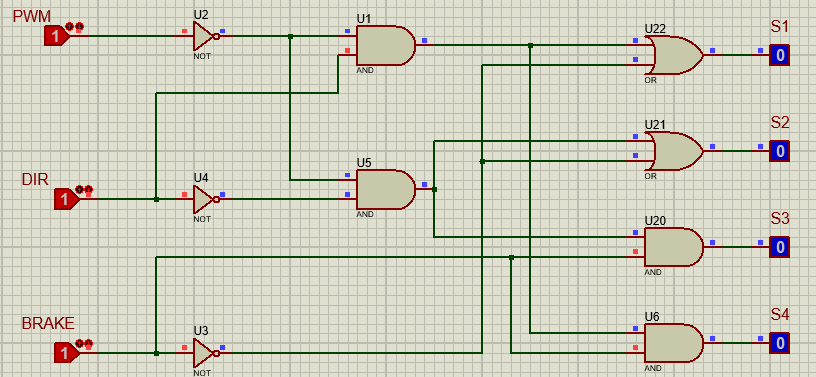
\includegraphics[width=0.6\textwidth]{pictures/3_result4.png}
                    \caption{Trường hợp 4: PWM1 = 1, PWM2 = 1, BRAKE = 1}
                \end{figure}
        \end{itemize}
        $\Rightarrow$ Kết quả mô phỏng đúng với bảng trạng thái tín hiệu các biến.
        
    
       